% `template.tex', a bare-bones example employing the AIAA class.
%
% For a more advanced example that makes use of several third-party
% LaTeX packages, see `advanced_example.tex', but please read the
% Known Problems section of the users manual first.
%
% Typical processing for PostScript (PS) output:
%
%  latex template
%  latex template   (repeat as needed to resolve references)
%
%  xdvi template    (onscreen draft display)
%  dvips template   (postscript)
%  gv template.ps   (onscreen display)
%  lpr template.ps  (hardcopy)
%
% With the above, only Encapsulated PostScript (EPS) images can be used.
%
% Typical processing for Portable Document Format (PDF) output:
%
%  pdflatex template
%  pdflatex template      (repeat as needed to resolve references)
%
%  acroread template.pdf  (onscreen display)
%
% If you have EPS figures, you will need to use the epstopdf script
% to convert them to PDF because PDF is a limmited subset of EPS.
% pdflatex accepts a variety of other image formats such as JPG, TIF,
% PNG, and so forth -- check the documentation for your version.
%
% If you do *not* specify suffixes when using the graphicx package's
% \includegraphics command, latex and pdflatex will automatically select
% the appropriate figure format from those available.  This allows you
% to produce PS and PDF output from the same LaTeX source file.
%
% To generate a large format (e.g., 11"x17") PostScript copy for editing
% purposes, use
%
%  dvips -x 1467 -O -0.65in,0.85in -t tabloid template
%
% For further details and support, read the Users Manual, aiaa.pdf.


% Try to reduce the number of latex support calls from people who
% don't read the included documentation.
%
\typeout{}\typeout{If latex fails to find aiaa-tc, read the README file!}
%


\documentclass[]{aiaa-tc}% insert '[draft]' option to show overfull boxes

\usepackage{graphicx}
\usepackage{xcolor}

 \title{Uncertainty Quantification Pertinent to Wind Farm Flow Physics and Modeling}

 \author{
    Pankaj K. Jha%
    \thanks{Senior Researcher, Wind Center of Excellence, Senior AIAA Member.},\\
   {\normalsize\itshape
   Envision Energy USA Ltd., Houston, TX 77002, USA}\\
    Aleksandar Jemcov%
    \thanks{Research Assistant Professor, Hessert Laboratory for Aerospace Research, AIAA Member.},\\
   {\normalsize\itshape
   University of Notre Dame, St. Joseph Drive, South Bend, IN, 46637, USA}\\
    Chris Sideroff%
    \thanks{Principal Director.},\\
   {\normalsize\itshape
   Applied CCM, Inc., 2125 Dutton Cr, Ottawa, ON, Canada K1J 6K3}\\
    Kyle S. Hutchings%
   \thanks{Senior Researcher, Wind Center of Excellence.},\
    Gregory S. Oxley%
   \thanks{Senior Manager, R \& D, Wind Center of Excellence.},\\
  {\normalsize\itshape
   Envision Energy USA Ltd., Houston, TX 77002, USA}\\
 Guolei Wang%
   \thanks{Staff Engineer.},\\
  {\normalsize\itshape
   Envision Digital, No. 1065 West Zhongshan Road, Changning District, Shanghai, China}\\
  \and
  Sven Schmitz %
   \thanks{Associate Professor, Department of Aerospace Engineering, Senior AIAA Member.}\\
  {\normalsize\itshape
  The Pennsylvania State University, University Park, PA 16802, USA}
 }

 % Data used by 'handcarry' option if invoked
 \AIAApapernumber{YEAR-NUMBER}
 \AIAAconference{Conference Name, Date, and Location}
 \AIAAcopyright{\AIAAcopyrightD{YEAR}}

 % Define commands to assure consistent treatment throughout document
 \newcommand{\eqnref}[1]{(\ref{#1})}
 \newcommand{\class}[1]{\texttt{#1}}
 \newcommand{\package}[1]{\texttt{#1}}
 \newcommand{\file}[1]{\texttt{#1}}
 \newcommand{\BibTeX}{\textsc{Bib}\TeX}

\begin{document}

\maketitle

\begin{abstract}
This paper attempts to identify and quantify the uncertainties associated with the modeling of wind farm and flow physics in wind farms. Different aspects and types of uncertainties in modeling the atmosphere and rotor using different fidelity methods are explained. A description of the uncertainty quantification algorithms is also presented. This is followed by some case studies of the identification and quantification of relevant uncertainties. The first one pertains to the input parameters and model constants for a wind resource assessment problem on a complex terrain. The second one explains the uncertainties associated with a turbine-turbine interaction problem in atmospheric boundary layer using different actuator line modeling approaches for rotors. This is further exemplified using the aleatoric and epistemic uncertainties in blade loads as a result of using actuator line method, followed by a discussion on the physical propagation of these uncertainties downstream. The third type of case study is that of a 3-D cosine hill where the polynomial chaos algorithm is applied to propagate the uncertainties in model constants for Reynolds-averaged Navier-Stokes equations and investigate their effect on the flow-field.    
\end{abstract}

\section*{Nomenclature}

\begin{tabbing}
  XXXXX \= \kill% this line sets tab stop
  $ADM$ \> Actuator disk method \\
  $ABL$ \> Atmospheric boundary layer \\
  $AEP$ \> Annual energy production \\
  $ALM$ \> Actuator line method \\
  $CF$ \> Capacity factor\\
  $COE$ \> Cost-of-energy \\
  $DES$ \> Detached-eddy simulation \\
  $\varepsilon$ \>Gaussian spreading width \\
  $GAD$ \> Generalized actuator disk \\
  $IFS$ \> Integrated forecast system \\
  $\kappa$ \> von Karman constant \\
  $L$ \> Monin-Obukhov length scale\\
  $LES$ \> Large-eddy simulation \\
  $NBL$ \> Neutral boundary layer \\
  $NREL$ \> National Renewable Energy Laboratory \\
  $q_{surf}$ \> Surface heat transfer rate \\
  $RANS$ \> Reynolds-averaged Navier-Stokes \\
  $SSC$ \> Stochastic simplex collocation \\
  $TI$ \> Turbulence intensity \\
  $TKE$ \> Turbulent kinetic energy \\
  $URANS$ \> Unsteady Reynolds-averaged Navier-Stokes \\
  $UQ$ \> Uncertainty quantification \\
  $WRA$ \> Wind resource assessment \\
  $WRF$ \> Weather research and forecasting\\
  $$ \>
 \end{tabbing}

\section{Introduction} \label{intro}
Though being one of the fastest growing sources of renewable energy, wind energy research faces a number of challenges today. One of the many difficulties involves an incomplete understanding of the turbine models and turbulence transport phenomena in a wind farm. This includes the understanding of atmospheric stability state, terrain, turbine modeling approaches, blade loads, fatigue, blade-loads-wake correlation, wake-wake and wake-atmospheric turbulence interaction.  Figure~\ref{f:HornsRev} shows the wake in Horns Rev [\textcolor{red}{Ref}] wind farm. An idea of the complexity of the problem can be gained from figure~\ref{f:HornsRev}. The complexity increases significantly in case of a complex terrain.

\begin{figure}
\centering
 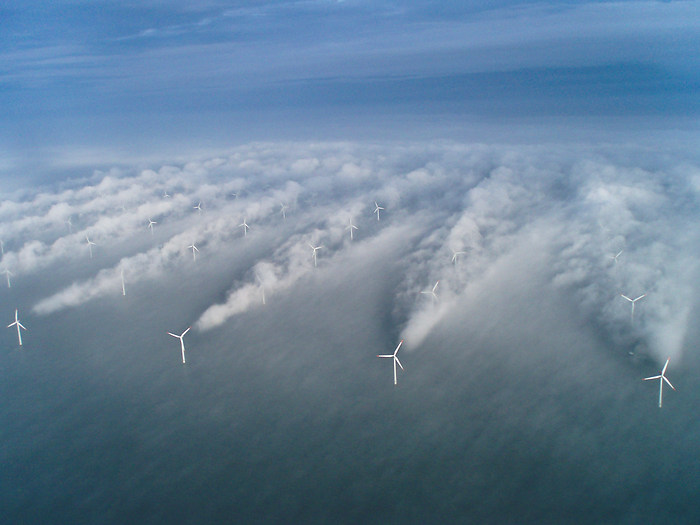
\includegraphics[width=0.65\textwidth]{HornsRev.png}
 \caption{Horns Rev Wind Farm.}
 \label{f:HornsRev}
\end{figure}

The associated array performance has a strong correlation with the spatial distance between turbines in an array. A well-designed utility-scale wind turbine can extract up to 50 percent of the wind power passing through its rotor disk area. The resulting viscous shear layer requires some distance to develop and to restore the momentum and energy that have been extracted by an upstream wind turbine. Moreover, the meandering of wakes from wind turbines from an adjacent row can cause span-wise shear in velocity and further complicate the flow field in front of a downstream turbine. Therefore, in the wind energy community, the accurate computation of the wake momentum deficit downstream of a wind turbine and its recovery are vital information for wind farm operators in order to correctly estimate the AEP. Improving array (or wind farm) performance while, at the same time, reducing blade fatigue loads are vital objectives towards reduced operation and maintenance (O \& M) costs and to an overall reduction in the cost-of-energy (COE) of wind-produced power. Meeting these objectives can be enabled by the quantification of associated uncertainties in the modeling chain and a better understanding of the different aspects of wind farm modeling mentioned above. Moreover, quantification of the uncertainties associated with the wind resource assessment (WRA) can help in planning a wind farm in the first place.

A true physical understanding of the subtleties involved in the operation of a wind farm is an open research problem. Wind farms operate under a range of atmospheric conditions and over a range of terrain. The goal of wind farm operators is to have the best possible assessment of wind resources for farm siting. They also need accurate blade loads and blade fatigue to understand the structural health and life span of wind turbines. A very good understanding of the complex flow physics invloving the interaction between wakes of different turbines and with the atmosphere is necessary to assess the array efficiency, capacity factor (CF), and annual energy production (AEP). Several state-of-the-art models for atmosphere, wind turbine rotors, and wakes exist. These models vary significantly in complexity and fidelity. It is very important to identify the most critical aspects of the modeling chain by quantifying the associated uncertainties such as atmospheric stability, boundary conditions, surface roughness, turbulence model, turbulence model parameters, turbine modeling approach, etc. This is necessary to define the range of applicability of these models and to develop the best practices guidelines under these uncertainties. These, in turn, will provide the farm operators the knowhow to optimize the AEP. 

This paper is organized as follows. Section \ref{uq_windfarm} explains the uncertainties pertinent to atmospheric modeling as well as rotor modeling. 
Section \ref{uq_algo} explains the algorithm used for propagation and quantification of uncertainties used for one of the case studies presented in \ref{cosineHill}. Section \ref{case_studies} explains three case studies:
\begin{itemize}
  \item Uncertainties in input parameters such as surface roughtness, surface heat flux, modeling of atmospheric stability, choice of turbulence models and model constants for a wind resource assessment problem on a complex terrain.
  \item Uncertainties associated with the flow physics of an array of turbines in an atmospheric boundary layer (ABL) using different actuator line model (ALM) approaches for rotors. The atmophere is modeled by large-eddy simulation (LES) and a flat terrain is considered for demeonstration where the focus is on ALM approaches. The relevant aleatoric and epistemic uncertainties in flow-field and blade loads as a result of using different ALM methods and their propagation is discussed.
  \item Uncertainties pertinent to a 3-D cosine hill where the standard algorithms such a polynomial chaos algorithm is used to progagate the uncertainties in model constants for Reynolds-averaged Navier-Stokes (RANS) equations and their effects on the flow-field are investigated.  
\end{itemize}
  
The paper concludes with some enhanced understanding of wind farms operating under these uncertainties that will help in better and effcient planning and operation of wind farms. Some suggestions are also presented for future work based on this study.

\section{Uncertainties in modeling a wind farm} \label{uq_windfarm}

Modeling of wind farm involves two steps. First, the atmosphere is modeled using some approach of choice. This involves dealing with the stability state, surface roughness etc. using some turbulence model. Depending on the choice of different parameters, uncertainties are involved with each of these to some extent. Understanding these uncertainties is a pre-requisite for efficient wind resource assessment.\cite{lackner:aiaa2007}\textsuperscript{, } \cite{lackner:asme2008}\textsuperscript{, } \cite{kwon:ae2010} Once the atmosphere has been modeled, turbines are modeled and coupled with the model for atmosphere. There are several approaches for modeling the turbines, each having their own source of uncertainties. The following sub-sections explain the two steps of modeling a wind farm and the associated uncertainties.

\subsection{Uncertainties in atmospheric modeling} \label{uq_abl}
Modeling of atmosphere is the first step in modeling a wind farm. There are different models for atmosphere such as weather research and forecasting (WRF)[\textcolor{red}{Ref}] and integrated forecast system (IFS)[\textcolor{red}{Ref}]. These models are for meso-scale weather phenomena where the length scales are on the order of several hundred kilometers. The length scales pertinent to wind farms (micro-scale) are much smaller than those dealt with by WRF and IFS. Therefore, in order to be able to use these models effectively for wind farm applications, a proper interpolation of relevant physical quantities between meso and micro scales must be done. Meso-micro coupling [\textcolor{red}{Ref}] is a very active area of research and beyond the scope of the current work. The most widely used approach to model the atmosphere for wind farm involves modeling the boundary layer where different layers of the ABL until the capping inversion are modeled. The capping inversion occurs at around 1 km above earth's surface. The length scales are on the order of wind turbines in a domain of several kilometers. This type of approach is implemented in National Renewable Energy Laboratory (NREL)'s SOWFA [\textcolor{red}{Ref}] code and Envision Energy's GWCFD code and forms the basis of discussion in this work.

Some of the key aspects of uncertainties pertinent to atmosphere modeling are discussed below:

\begin{itemize}
  \item \textit{The uncertainties associated with the choice of the turbulence model and flow solver:}

The ABL on a flat or complex terrain can be modeled by one of the different fidelity turbulence models and flow solver. This involves using Reynolds-averaged Navier Stokes (RANS), unsteady Reynolds-averaged Navier Stokes (URANS), detached-eddy simulation (DES), or large-eddy simulation (LES). Now, depending on how complex the terrain is and the primary wind direction, one model may capture better flow features than others. For example, DES can do a better job at resolving the flow features in the recirculating zone behind a hill. Moreover, the choice of the specific turbulence model, say $k-\omega$, $k- \epsilon$ or $k - \omega$  $SST$ and the model constants would lead to different accuracy of flow-field in the regions near the surface (surface layer) and low shear region of the ABL. Therefore, any further analysis based on the flow-field, such as computation of turbulence intensity (TI), AEP, wind shear, inflow angle etc. is subject to uncertainty in the flow-field. The uncertainty in the flow-field is, in turn, dependent on the choice of the flow model. This will be explained further in the case study presented in section \ref{case_wra}.
 
 \item \textit{The uncertainties associated with the choice of stability state of the atmosphere:}

Different stability states of the atmosphere during a diurnal cycle are characterized by different surface heating, $q_{surf}$. This is also associated with the Monin-Obukhov length scale, $L$. The stability state determines the mixing behavior and recovery of the momentum deficit in the wake of a turbine. The atmopsheric modeling code could take either $q_{surf}$ or $L$ as an input. The choice of the input is a source of uncertainty in ABL stability modeling, and hence in the flow-field and any analysis based on the flow-field, as mentioned in the above bullet.  

  \item  \textit{The uncertainties associated with the surface roughness:}

The choice of the roughness model, i.e., a variable roughness map or a constant roughness can significantly alter the wind profile. Moreover, even for constant roughness, the value of roughness not representative of the terrain and vegetation, can also alter the flow-field. Therefore, any analysis based on this is subject to uncertainty.
 
\end{itemize}

Apart from the items discussed above, other parameters that could lead to uncertainty in the flow-field include the mesh resolution along the surface, the mesh resolution in the vertical direction, the growth pattern of the mesh, the choice of representative von Karman cosntant, $\kappa$ etc.
 
\subsection{Uncertainties in rotor modeling}
As mentioned above, once the atmosphere has been modeled, the turbines are modeled and coupled with the models for atmosphere. There are several popular models for wind turbines (also applicabale to wings and other types of rotors such as helicopters, propellers, and tidal turbines). These include blade element momentum (BEM) method, actuator disk method (ADM), generalized actuator disk (GAD) method, actuator line method (ALM), actuator surface method (ASM) in increasing order of fidelity. Each of these methods have certain assumptions and parameters, and hence the blade loads and the intergated quantities such as power, thrust, and bending moment computed using these models are subject to uncertainty. For example, when modeling the rotor using BEM, the local inflow may not have been modeled correctly and hence will lead to an uncertain computation of blade loads, power etc. Moreover, the tip-loss model is another source of uncertainty. Likewise, when modeling the rotor using ADM or ALM, the choice of Gaussian spreading width, $\varepsilon$, is a source of uncertainty. The case study presented in section \ref{abl_alm} discusses the uncertainty associated with ALM.


\section{Algorithm for uncertainty propagation} \label{uq_algo}
Having given an overview of different aspects of UQ pertinent to wind farm in the preceding sections, this section explains the algorithm used for propagation of uncertainty. This algorithm is used in the case study on 3-D cosine hill presented in section \ref{cosineHill}

\subsection{Polynomial chaos}
 [\textcolor{red}{To be completed}]

\subsection{Any other algorithm used} 
[\textcolor{red}{To be completed}]

\section{Case studies} \label{case_studies}

This section presents some case studies of the identification and quantification of relevant uncertainties. The first one pertains to the input parameters and model constants for a wind resource assessment problem on a complex terrain. The second one explains the uncertainties associated with a turbine-turbine-atmosphere interaction problem in atmospheric boundary layer using different actuator line modeling approaches for rotors. The third one explains a 3-D cosine hill where the polynomial chaos algorithm is applied to propagate the uncertainties in model constants for Reynolds-averaged Navier-Stokes equations and their effect on the flow-field are investigated.

\subsection{Wind resource assessment on complex terrain} \label{case_wra}
This case study is presented for two actual wind sites and follows the discussion in section \ref{uq_abl}. The wind sites chosen for this case study are Chongli [\textcolor{red}{Ref}] and Xuan Cheng  [\textcolor{red}{Ref}] in China. 

\subsubsection{Chongli wind site} \label{Chongli}

A subset of the terrain map of Chongli site is shown in figure \ref{f:Chongli_Terrain}. Some turbine locations are also shown for reference, though they are not used in this study. It can be noted that this site has quite complex terrain. The elevation above sea level varies from 1,100 meters to 1,700 meters. 

\begin{figure}
\centering
 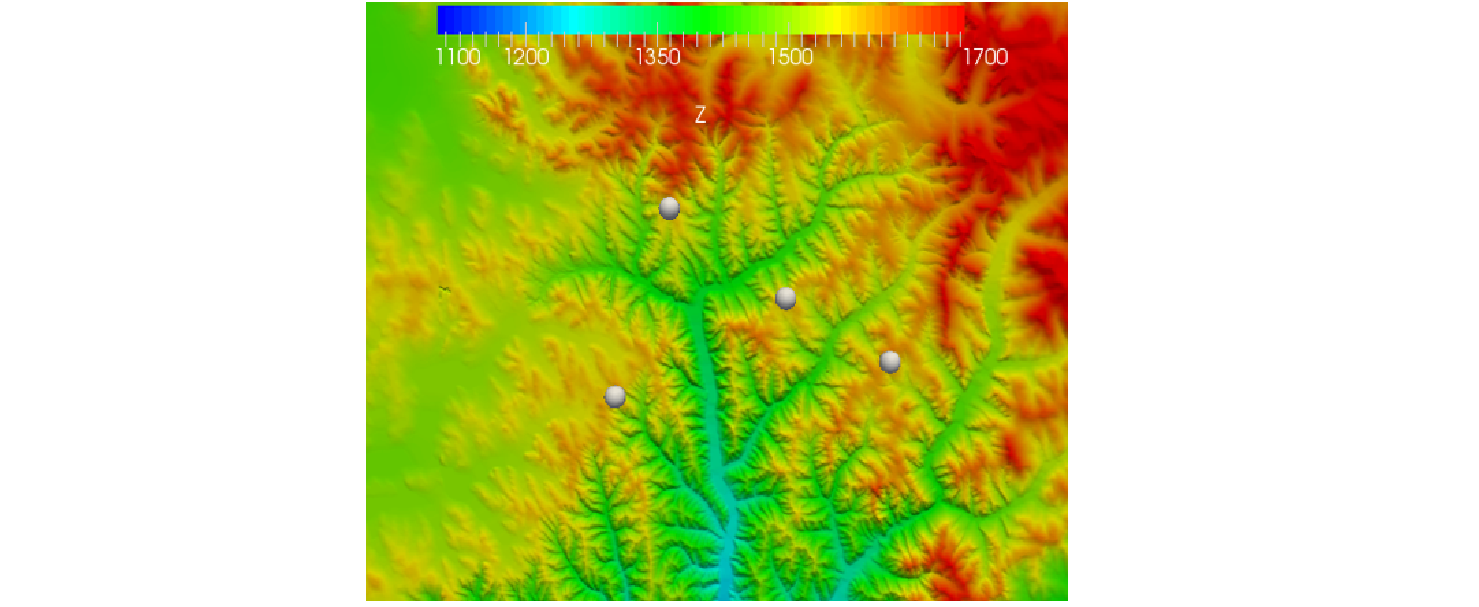
\includegraphics[width=1.05\textwidth]{Chongli_Terrain.png}
 \caption{Terrain map of Chongli wind site.}
 \label{f:Chongli_Terrain}
\end{figure}

Since this site has quite complex terrain, RANS modeling was deemed not suitable for resolving important flow features in the recirculation zone behind a hill. A DES  $k - \omega$  $SST$ turbulence model and neutral ABL atmospheric stability model were used. Figure \ref{f:DES_ComplexTerrain} shows two different zooms of the flow-field for this site. Isocontours of the horizontal wind speed are shown. The recirculation zone can be clearly seen. As discussed in section  \ref{uq_abl}, the site is prone to uncertainties associated with stability of the atmosphere and turbulence model. A variable surface roughness was used, that is also a source of uncertainty. Therefore, any further analysis based on the flow-field, such as computation of TI, AEP, wind shear, inflow angle etc. is subject to uncertainty in the flow-field.

\begin{figure}
\centering
 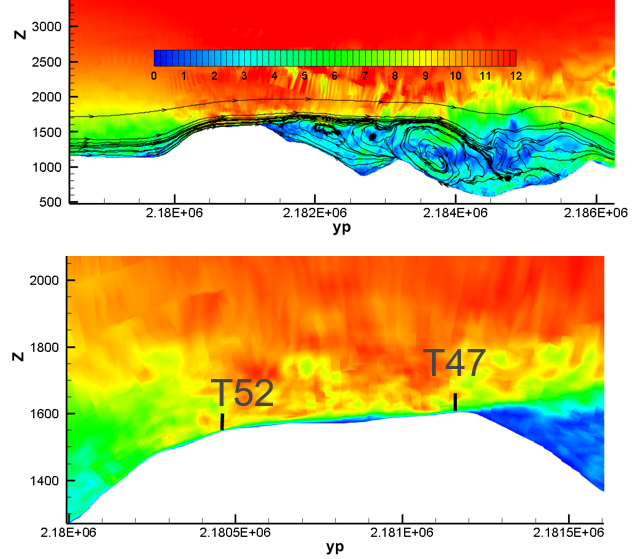
\includegraphics[width=0.65\textwidth]{DES_ComplexTerrain.png}
 \caption{Detached-eddy simulation for Chongli wind site.}
 \label{f:DES_ComplexTerrain}
\end{figure}

\subsubsection{Xuan Cheng wind site: uncertainty in turbulence model constant}

A qualitative discussion of the uncertainties associated with WRA was presented in the section \ref{Chongli}. This section discusses about the effect of choice of turbulence model constants. Xuan Cheng wind site is chosen for the case study. This site is relatively simpler compared to Chongli, so RANS $k - \epsilon$  turbulence model and neutral ABL atmospheric stability model were used. A variation of the model parameter $C_1$ of the $k - \epsilon$  turbulence model was done to investigate its effect on the flow-field. Figure \ref{f:XuanCheng_C1} shows the flow field from two different sections of the wind site, each with value of $C_1$ = 1.44 and 1.14. It can be observed from the flow-field that the variation in $C_1$ does lead to different flow-fields. Therefore, any uncertainty in $C_1$ is expected to lead to uncertainty in AEP, wind shear, etc. A formal UQ study involving the propagation of uncertainty using polynomial chaos algorithm for a 3-D cosine hill is presented in section \ref{cosineHill}.

\begin{figure}
\centering
 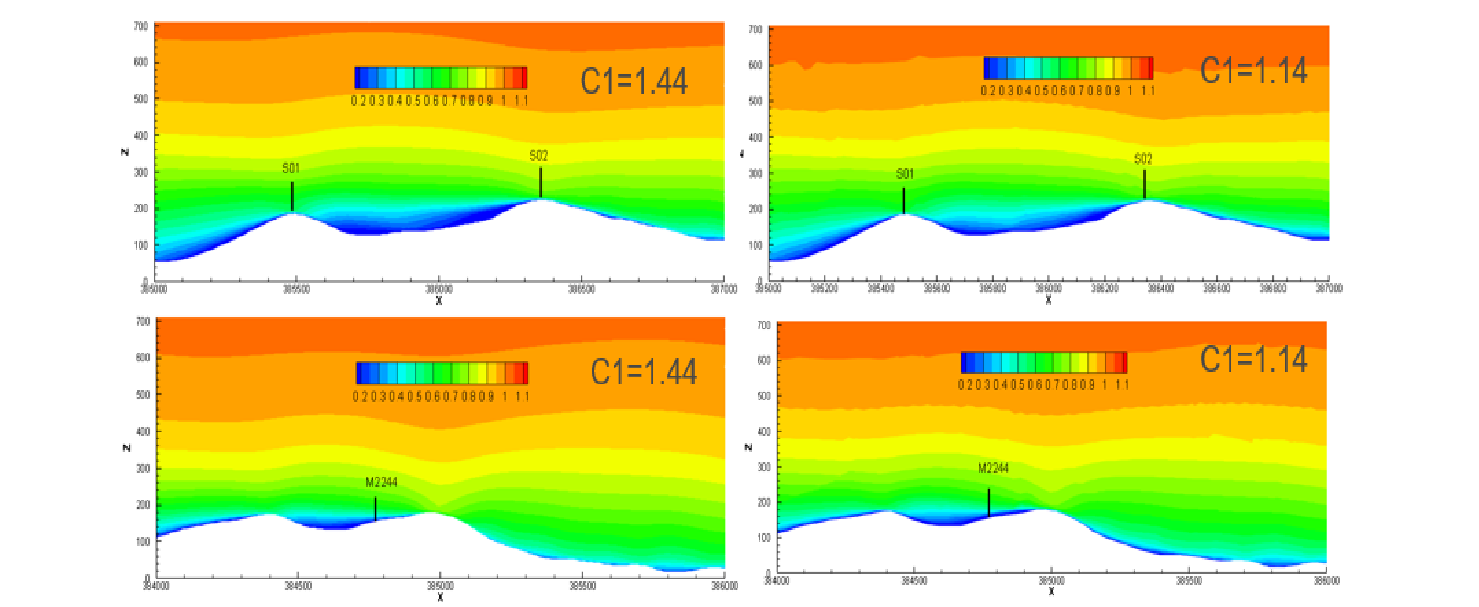
\includegraphics[width=0.85\textwidth]{XuanCheng_C1_Effect.png}
 \caption{Effect of the RANS model constant $C_1$ for Xuan Cheng wind site.}
 \label{f:XuanCheng_C1}
\end{figure}


\subsection{Turbine-turbine-atmosphere interaction problem using actuator line method} \label{abl_alm}

This case study explores the uncertainties associated with the turbine model coupled with atmosphere model. 
The ALM coupled with LES of the ABL, has evolved as the technology standard in the wind energy community for modeling the rotor, fatigue, and wakes of standalone as well as an array of wind turbines immersed in an ABL flow. This study discusses a turbine-turbine-atmosphere interaction problem from the recent work by the leading author.\cite{jha:aiaa2014}\textsuperscript{, }\cite{jha:jsee2014} This work has demonstrated the effect of different ALM modeling approaches and ABL state on turbulence statistics and unsteadiness of blade loads, as well as power and wake profile for a turbine-turbine interaction problem. It was noted in this study that extending this work to a wind farm and a detailed study on the quantification of these and other uncertainties would be a major enhancement in the state-of-the-art in wind energy research. The uncertainties in the ABL inflow and in the physical quantities such as blade loads, as a result of modeling parameters in the ALM, augment the uncertainty in the prediction of velocity (or power available in the wind), blade loads, integrated power, wake meandering etc. at a downstream location and in other rows. This is addressed in the following section where a discussion on the identification of these uncertainties is presented.

As noted above, the uncertainties arising due to atmosphere and rotor modeling should be formally quantified. These uncertainties could be identified as those due to long-term wind forecast, diurnal wind forecast, wind farm inflow, rotor modeling, wake turbulence, etc. In this section, two types of uncertainties, viz., aleatoric and epistemic, will be discussed for the example problem mentioned above. 

\subsubsection{Aleatoric uncertainties}

The example problem under consideration is essentially influenced by uncertainties. The ABL is modeled using an LES approach\cite{churchfield:aiaa2012} using several parameters such as surface roughness, surrface heat flux, surface roughness, etc. as inputs. These inputs are the sources of uncertainties in ABL modeling as discussed in section \ref{uq_abl}

It is noteworthy that the different radial locations of a turbine operating under such a condition experience different inflow. Moreover, the transients in the inflow conditions add to the uncertainty in the inflow condition. The modeling errors in ABL are epistemic in nature, if the flow under consideration is ABL only, for example in the case of WRA. However, since the ABL inflow is an input for wind turbine/farm simulation, the uncertainties in the prediction of inflow to the turbines can be considered aleatoric. These uncertainties are functions of ABL model parameters. Figure~\ref{f:UQ1} shows the eddy structures (iso-surfaces of velocity fluctuations) for a standalone ABL simulation. The ABL modeling parameters lead to uncertainty in the velocity shear and hence in the vorticity and the prediction of eddy structures.

\subsubsection{Epistemic uncertainties}

The results of the ABL simulation serve as inflow to the wind farm simulation. For a given inflow condition (with inherent aleatoric uncertainties), when a blade is modeled using ALM, the prediction of blade loads depends on ALM parameters. Jha et. al. \cite{jha:aiaa2014}\textsuperscript{, }\cite{jha:jsee2014} have shown that the different ALM approaches result in different predicted blade loads for the outermost 15 \% of the span. The consequent difference in the integrated power can be on the order of 4-5 \% for the downstream turbine. Moreover, the differential lift along the span determines the circulation, hence the strength of the tip vortices is determined by the blade load distribution along the outer portion of blade span, which in turn depends on the ALM approach. The tip vortices advect downstream and break down and characterize the flow downstream. So the error induced due to modeling in the blade loads affects the wake profile and the inflow to the downstream turbine. Thus the epistemic uncertainty in the blade loads (and consequently tip vortices) for the upstream turbine results in the aleatoric uncertainty for the downstream turbine in addition to the aleatoric uncertainty in the ABL. Figure~\ref{f:ALM_discrepancy} shows the epistemic uncertainty in the blade loads (near tip) for the two turbines and Figure \ref{f:UQ3} shows the aleatoric uncertainty in the inflow to the downstream turbine.

\begin{figure}
\centering
 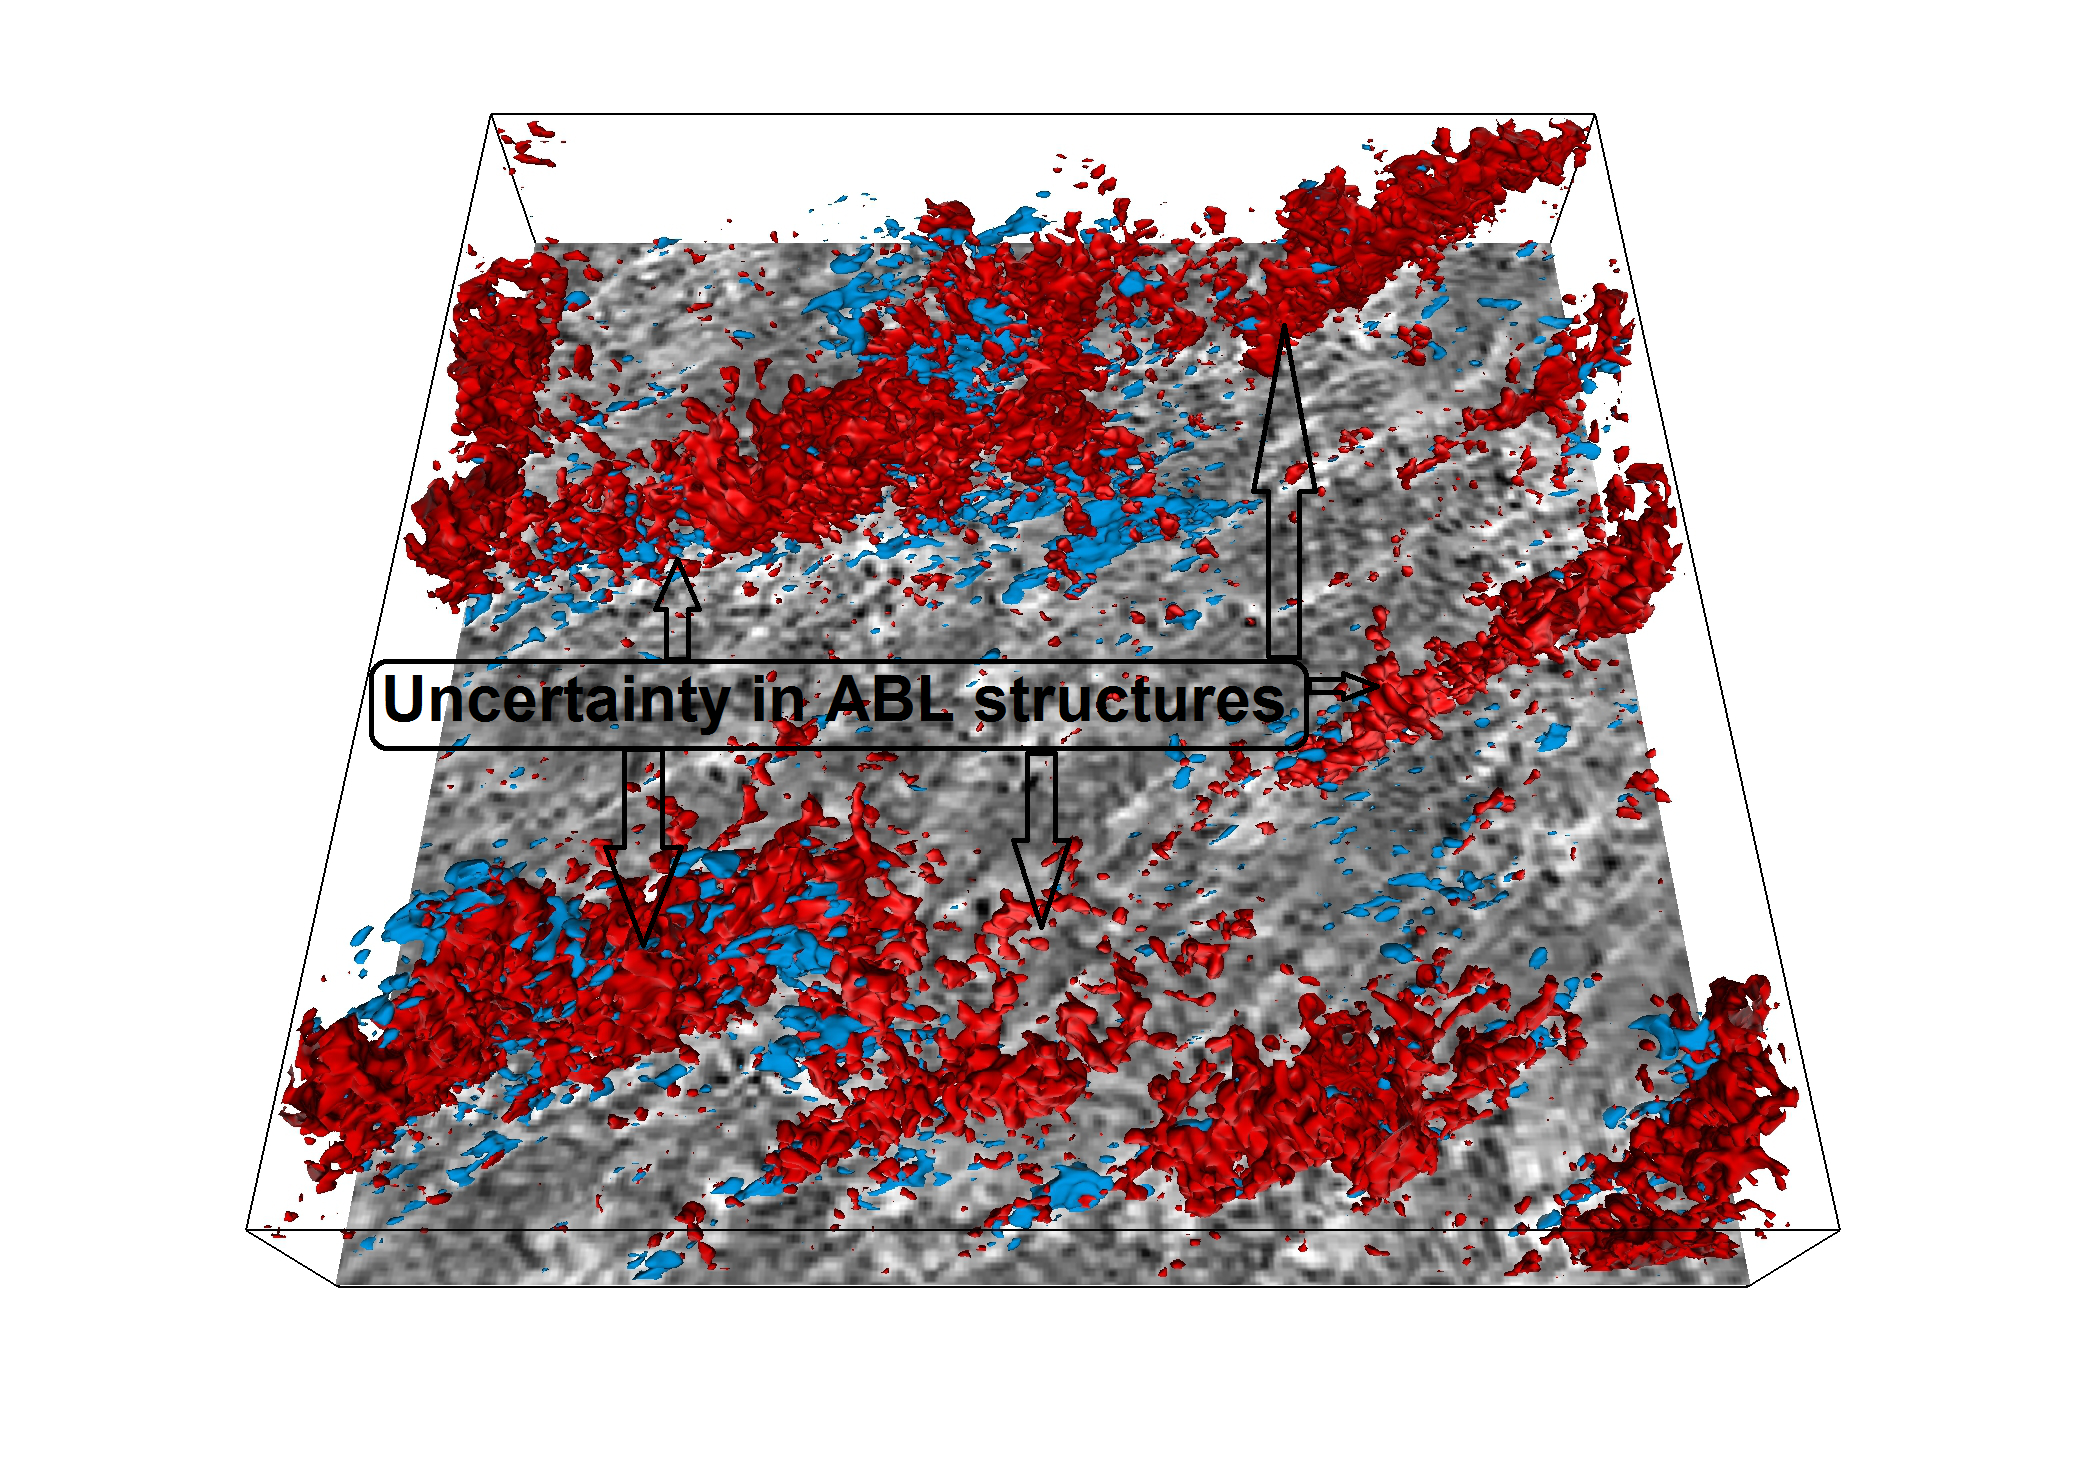
\includegraphics[width=0.75\textwidth]{UQ1.png}
 \caption{Iso-surface of instantaneous velocity fluctuations and aleatoric uncertainties.}
 \label{f:UQ1}
\end{figure}

\begin{figure}
\centering
 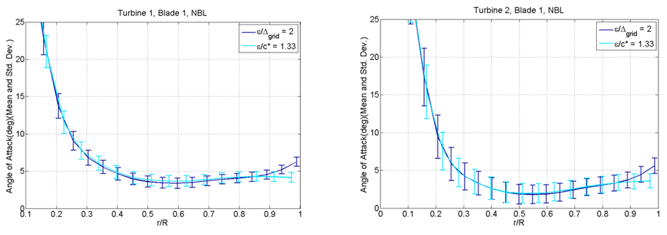
\includegraphics[width=0.85\textwidth]{ALM_discrepancy.png}
 \caption{Epistemic uncertainties in mean angle-of-attack (AOA). (a) Turbine 1 (NBL)    (b) Turbine 2 (NBL).}
 \label{f:ALM_discrepancy}
\end{figure}

\begin{figure}
\centering
 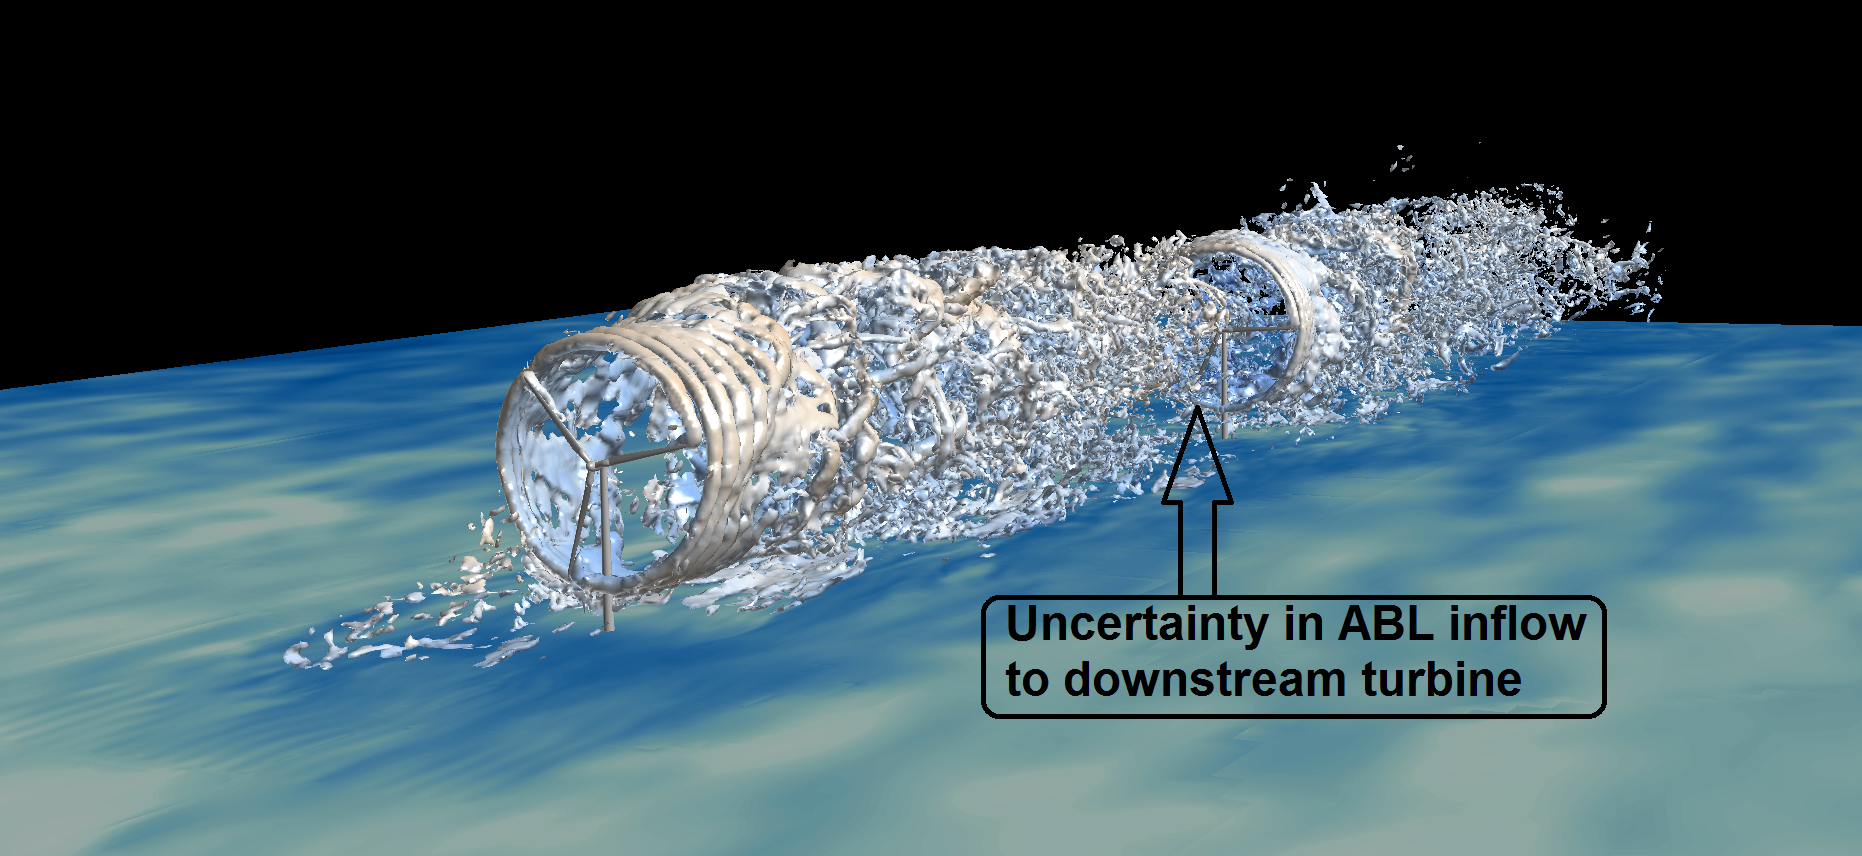
\includegraphics[width=0.75\textwidth]{UQ3.png}
 \caption{Uncertainties in the wake and inflow (aleatoric) to the downstream turbine.}
 \label{f:UQ3}
\end{figure}

From the above discussion of a turbine-turbine interaction problem, we can summarize the uncertainties identified so far:

Upstream turbine: 
\begin{itemize}
  \item Aleatoric uncertainty due to ABL (spatial and temporal variations).
  \item Epistemic uncertainty in the predicted blade loads and derived quantities such as power.
\end{itemize}

Downstream turbine: 
\begin{itemize}
  \item Aleatoric uncertainty due to ABL (spatial and temporal variations, which depend on ABL state), and the epistemic uncertainty in the blade loads (tip vortices) of the upstream turbine which have propagated in the wake, depicted in figure \ref{f:UQ3}.
  \item Epistemic uncertainty in the predicted blade loads and derived quantities such as power.
\end{itemize}

From this simple model of two turbines we can infer that, in a real wind farm with multiple turbines (could be around 50-100), the aleatoric uncertainty in inflow at a downstream turbine is the accumulation of epistemic uncertainty in the blade loads of all the upstream turbines. For a real wind farm, such as Lillgund,\cite{churchfield:aiaa2012} the accumulated uncertainties in the blade loads, power prediction, and wake profiles are anticipated to be much more pronounced than that discussed for the two-turbine example. Since these uncertainties are directly related to the structure and strength of the tip vortices, which determine the wake recovery process, the problem described needs a detailed investigation for a real wind farm.

In addition to the sources of uncertainties identified above, wake meandering can cause a severe wind shear in the horizontal and spanwise directions. Hence, the wake from a turbine and any epistemic uncertainty associated with it adds to the aleatoric uncertainty of each turbine affected by wake meandering. An idea of the advection of uncertainties and wake meandering can be obtained from Figure \ref{f:UQ2}. It shows the flow-field of an array of five NREL 5-MW turbines, where the main row comprises three turbines and the sub-row comprises two. The iso-surface of vorticity magnitude 0.5 1/s is shown on the left and the iso-surface of velocity fluctuations (u’ = 2.5 m/s (blue), w’ = 2.0 m/s (red)) on the right. 

\begin{figure}
\centering
 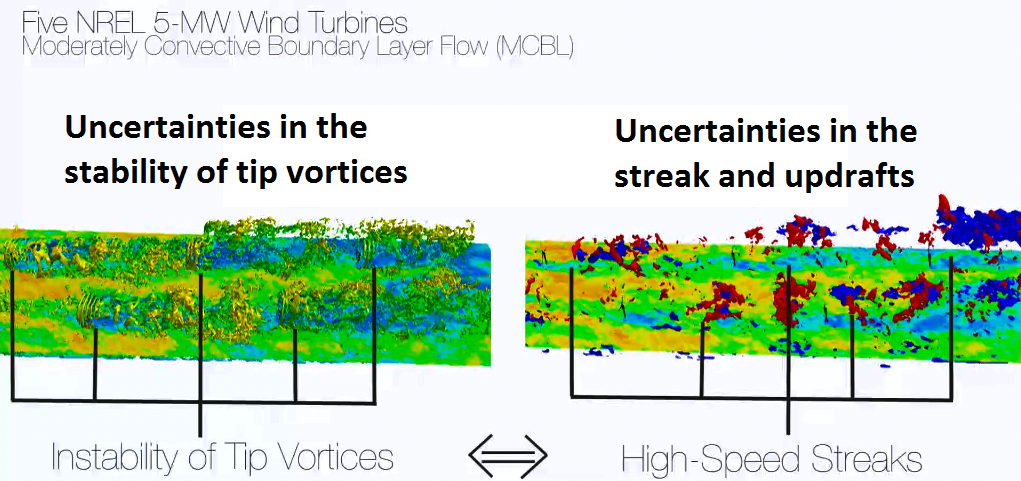
\includegraphics[width=0.85\textwidth]{UQ2.png}
 \caption{Uncertainties in tip vortices, streaks, and updrafts in a turbine array.}
 \label{f:UQ2}
\end{figure}

\subsection{3-D Cosine hill using RANS and polynomial chaos} \label{cosineHill}
From the above two case studies we got plenty of idea on the sources and types of uncertainty. However, before attempting to quantify those uncertainties in an actual wind farm, it is wise to work on a model problem which has characteristics of the main problem at hand but is not that complicated. As such, a 3-D cosine hill was chosen to be the model problem. The flow feautures are similar to a complex terrain, however, the flow is smoother.  This model problem is focused on WRA.  RANS $k - \epsilon$  turbulence model and neutral ABL atmospheric stability model were used.
A UQ study was performed by varying the model constant $C_{\mu}$. The geomtery of the model problem is shown in figure \ref{f:cosine_hill}

\begin{figure}
\centering
 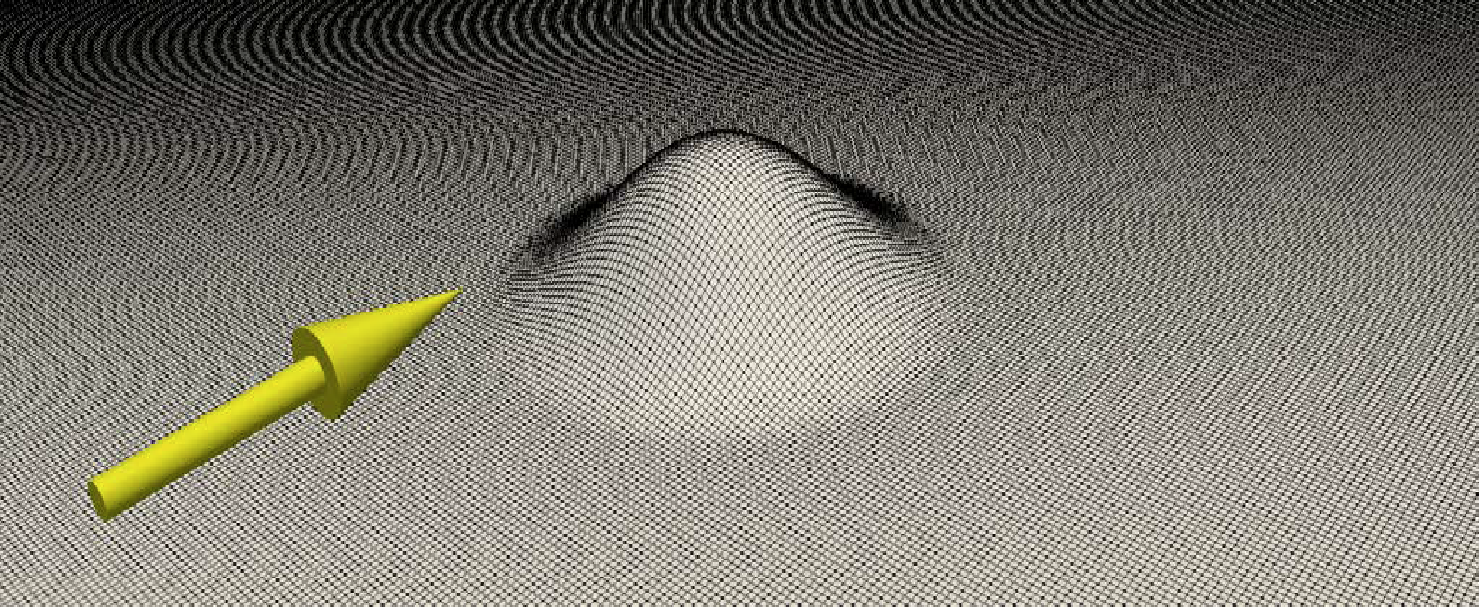
\includegraphics[width=0.85\textwidth]{CosineHill.png}
 \caption{3-D Cosine hill used for uncertainty quantification study. [\textcolor{red}{ Replace with a nicer figure if possible.}] }
 \label{f:cosine_hill}
\end{figure}

[\textcolor{red}{To be completed}]

\section{Conclusions and future work}
[\textcolor{red}{To be written based on the final paper.}]
Several uncertainties pertinent to wind farm were identified. A formal study was undertaken to.....



\textbf{Acknowledgment}

\begin{thebibliography}{9}% maximum number of references (for label width)

\bibitem{bib_message}
[\textcolor{red}{More references to be added, some redundant ones to be removed.}]

\bibitem{lackner:aiaa2007}
Lackner, M.A., Rogers, A.L., and Manwell, J.F., ``Uncertainty Analysis in Wind Resource Assessment and Wind Energy Production Estimation," AIAA 2007-1222.

\bibitem{lackner:asme2008}
Lackner, M.A., Rogers, A.L., and Manwell, J.F., ``Uncertainty Analysis in MCP-Based Wind Resource Assessment and Energy Production Estimation," ASME Journal of Solar Energy Engineering, 130(3), 031006 (Jul 01, 2008).

\bibitem{kwon:ae2010}
Kwon, S.D., ``Uncertainty analysis of wind energy potential assessment," Applied Energy, 87(3), pp 856-865.

\bibitem{jha:aiaa2014}
Jha, P. K., Churchfield, M. J., Moriarty, P. J., and Schmitz, S., ``The Effect of Various Actuator-Line   Modeling Approaches on Turbine-Turbine Interactions and Wake-Turbulence Statistics in Atmospheric Boundary-Layer Flow," AIAA 2014-0710.

\bibitem{jha:jsee2014}
Jha, P. K., Churchfield, M. J., Moriarty, P. J., and Schmitz, S., ``Guidelines for Volume Force  Distributions within Actuator Line Modeling of Wind Turbines on Large-Eddy Simulation-type Grids," ASME Journal of Solar Energy Engineering, 136(3), 0310014 (Jan 10, 2014).

\bibitem{churchfield:aiaa2012}
Churchfield, M. J., Lee, S., Moriarty, P. J., Martínez, L. A., Leonardi, S., Vijayakumar, G. and  Brasseur, J. G., ``A Large-Eddy Simulation of Wind-Plant Aerodynamics," AIAA 2012-0537.

\bibitem{iman:wiley2008}
Iman, R. L., ``Latin Hypercube Sampling," Encyclopedia of Quantitative Risk Analysis and Assessment, Wiley 2008

\bibitem{helton:re2003}
Helton, J.C. and Davis, F.J., ``Latin hypercube sampling and the propagation of uncertainty in analyses of complex systems," Reliability Engineering \& System Safety, 81(1), pp 23-69

\bibitem{witterveen:aiaa2010}
Witterveen, J.A.S. and Iaccarino, G., ``Simplex Elements Stochastic Collocation in Higher-Dimensional Probability Spaces." AIAA 2010-2924

\bibitem{witterveen:siam2012}
Witterveen, J.A.S. and Iaccarino, G., ``Simplex Stochastic Collocation with Random Sampling and Extrapolation for Nonhypercube Probability Spaces," SIAM J. Sci. Comput., 34(2), pp A814–A838.

\bibitem{witterveen:jcp2013}
Witterveen, J.A.S. and Iaccarino, G., ``Simplex stochastic collocation with ENO-type stencil selection for robust uncertainty quantification, Journal of Computational Physics, Volume 239, 15 April 2013, pp 1-21.

\bibitem{najm:arfm2009}
Najm, H. N., ``Uncertainty Quantification and Polynomial Chaos Techniques in Computational Fluid Dynamics," Annual Review of Fluid Mechanics
Vol. 41, pp 35-52. 


\end{thebibliography}

\end{document}

% - Release $Name:  $ -
